%        File: dupa.tex
%     Created: wt  lut 16 04:00  2010 C
% Last Change: pon mar 01 04:00  2010 C
%
\documentclass[a4paper]{article}
\usepackage[pdftex]{graphicx}
\usepackage[utf8]{inputenc}
\usepackage[polish]{babel}
\usepackage[T1]{fontenc}
\begin{document}

\section{Wpływ zmiany parametrów definiowania klas ruchowych w DiffServ na transmisję w sieci}

Projekt z przedmiotu Gwarantowanie Jakości Obsługi w Internecie

Jacek Szarski
Mateusz Zawisza


Naszym zadaniem było znalezienie związku pomiędzy konfiguracją mechanizmu DiffServ a uzyskaną jakością obsługi. W tym celu przygotowaliśmy symulację niedużej sieci IP z implementacją owego systemu, a następnie analizowaliśmy wyniki uzyskan dla różnych zadanych ustawień.


\section{Topologia sieci}

%obrazek z topologią
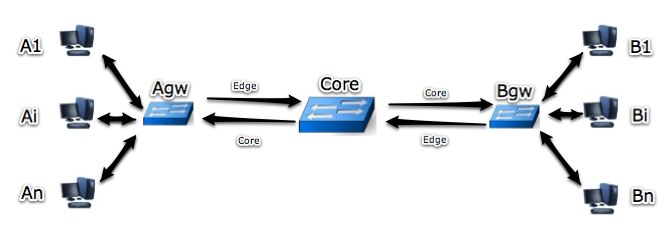
\includegraphics[width=120mm]{images/topologia.jpeg}

\paragraph{}
W zestawionej przez nas sieci znajdowały się trzy węzły stanowiące źródła ruchu (A1, A2 ,A3), oraz trzy węzły będące odbiorcami ruchu (B1, B2, B3). Transmisja odbywała się od każdego nadawcy do każdego odbiorcy. Symulacja została ustawiona tak aby wystąpiły przeciążenia sieci na odcinku Agw - Bgw, co wiąże się z utratą przesyłanych pakietów.

\paragraph{}
Zastosowaliśmy politykę DiffServ Time Sliding Window Three Color Marker (TSW3CM).
Polityka ta przyjmuje dwa parametry: CIR oraz PIR. Na ich podstawie oznacza pakiety kolorami zielony, żółty oraz czerwony. Pakiety które mieszczą się pod progiem CIR znaczone są na zielono, te które mieszczą się pomiędzy CIR oraz PIR znaczone są na żółto oraz te które są ponad progiem PIR znaczone są na czerwono. U nas przekładają się ona na wirtualne kanały, odpowiednio 0,1 oraz 2 co też wiąże się z odpowiednimi priorytetami. Najmniejszy priorytet mają pakiety w kanale wirtualnym 2 , a największy w kanale 0.


\section{Szczegóły techniczne}


\paragraph{}
Symulację napisaliśmy w języku TCl, dla symulatora NS (plik router.tcl), a następnie, aby zautomatyzować proces gromadzenia danych, stworzyliśmy bibliotekę napisaną w języku Ruby która uruchamia go z zadanymi parametrami (simulation.rb). Część parametrów przekazywane jest przez zmienne środowiskowe środowiska BASH, część zaś przez plik tekstowy queue\_params. Cały program znajduje się w pliku program.rb.


\section{Czas rozbiegu}

\paragraph{}
Aby ustalić czas rozbiegu symulacji badaliśmy ilość zrzucanych ramek w czasie. Zayliśmy że w większości przypadków po ok 1/4 czasu trwania danej symulacji wyniki zaczynają się stabilizować. Po około 3/4 czasu trwania znów pojawia się zmiana w tendencji. Postanowiliśmy zatem ograniczyć czas pobierania wyników do zakresu od 1/4 do 3/4 czasu trwania.

\paragraph{}
Symulator co 0.1 sekundy zwraca tabelę ze statystykami łącza. Wszystkie te tabele parsujemy, wybieramy wyniki w okolicach granic czasowych i odejmujemy je od siebie. W ten sposób faza rozbiegu oraz zakańczania nie mają wpływu na naszą analizę.


\section{eksperyment 1 - Prawdopodobieństwa zrzutu}



\subsection{parametry symulacji:}

Rozmiar pakietów (packet size) - 1000 KB
Ilość przepływów (flows count) - 100
Przepustowość wszystkich łączy (throughput) - 4Mb 
CIR (commited information rate) pasmo zapewnione - 30 kb/s
PIR (peak information rate) pasmo szczytowe - 60 kb/s
Średnie opóźnienie pomiędzy wysyłanymi pakietami - 0.01 s

\subsection{analiza:}

\paragraph{}
W poszczegulnych symulacjach zmienialiśmy wartości prawdopodobieństw zrzutu pakietów odpowiednio dla punktów kodowych 10, 11, 12, odpowiadającym kolorom zielonemu, żółtemu i czerwonemu.
Przeciążenie łącza pozwoliło nam na zbadanie ilości pakietów zrzuconych przez DiffServ (edrops) oraz ilość pakietów zrzuconych z powodu przeciążenia łącza (ldrops) dla różnych prawdopodobieństw zrzutu w odpowiednich kanałach.

\paragraph{}
Ilość pakietów wysyłanych w ciągu sekundy przez węzły powoduje bardzo szybkie przekroczenie wartości CIR i PIR. Większość pakietów w związku z tym zostaje oznaczona kolorem czerwonym i posiada najniższy priorytet. Dlatego znaczenie praktycznie ma tylko prawdopodobieństwo zrzutu dla pakietów oznaczonych kolorem czerwonym. 

\paragraph{}
Chcielibyśmy aby zrzucanie pakietów w większości dokonywane było przez DiffServ, gdyż w ten sposób zrzucane w pierwszej kolejności będą pakiety z najmniejszym priorytetem. Pakiety które zrzucane są z powodu przeciążenia łącza (ldrop) są pakietami losowymi i nie możemy w takiej sytuacji zapewnić zadanych parametrów QoS.

\paragraph{}
Badając ilość paketów które dotarły oraz stosunek ilości edropów do ldropów zauważylimy ścisłą korelację pomiędzy prawdopodobieństwem zrzutu kolojki czerowonej a sposobem zrzucania pakietów.

\paragraph{}
Zmiany pozostałych prawdopodobieństw nie miały wpływu na wyniki, przedstawiamy więc tylko ich wybraną część, która ilustruje związek.


%wykres z prawdopodobieństwami
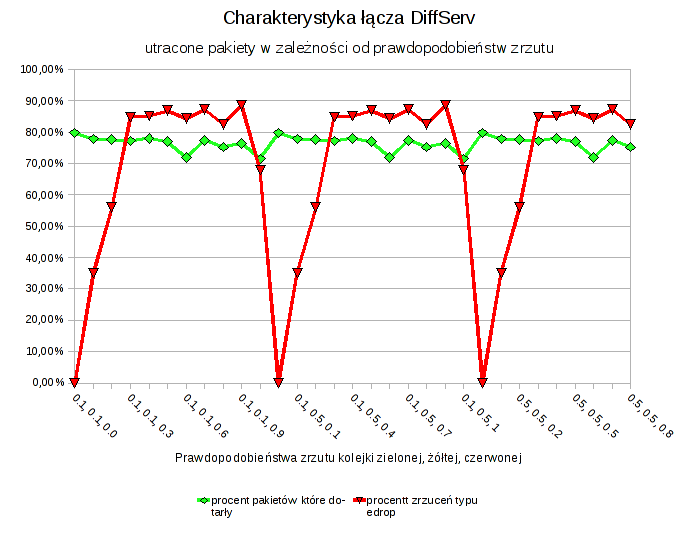
\includegraphics[width=120mm]{images/punkt_1_wykres.png}


% TABELKA
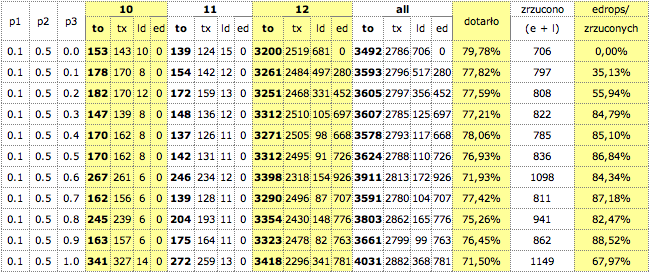
\includegraphics[width=120mm]{images/punkt_1_tabela.png}

\paragraph{}
Procent edropów który przyjeliśmy za wyznacznik jakości łącza przyjmuje najwyższe wartości dla prawdopodobieństwa p3 z zakresu 0,3 do 0,9. Dla tego przedziału procent pakietów które dotarły do swojego przeznaczenia największą wartość osiąga dla p3=0,4, zatem tą wartość moglibyśmy uznać za najbardziej odpowiednią dla naszej topologii. 

\paragraph{}
Minimalna wartość ldropów w kolejce zielonej wystąpiła dla p3=0,6 i wynosiła 2,25\%. Przy tak małych wartościach ciężko jednak uznać tą wartość za reprezentatywną.



\section{eksperyment 2 - Kolejkowanie pakietów}

\subsection{parametry symulacji:}

rozmiar pakietu: 100B\\
średni rozmiar pliku: 200kB\\
ilość przepływów: 100\\
przepustowość łącza: 6kb\\
średni odstęp pomiędzy początkami transmisji: 0.3s\\
CIR oraz PIR były zmiennymi\\
\subsection{analiza:}

\paragraph{}
W celu zobrazowania zasady działania kolejek diffserva przeprowadziliśmy symulacje przy zmieniających się parametrach CIR i PIR. PIR był zawsze dwa razy większy od CIR.
Na wykresie poniżej możemy zaobserwować w jaki sposób pakiety przydzielane są do poszczególnych kolejek.\\
\\



%wykres z kolejkami
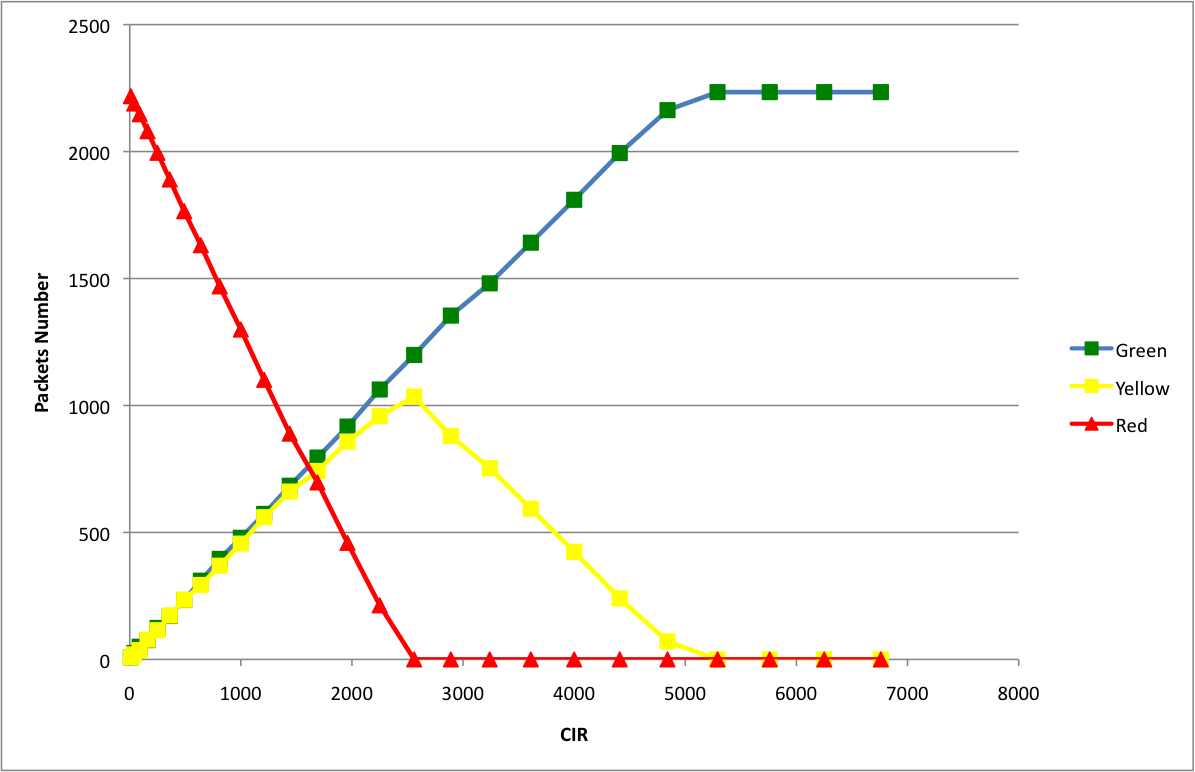
\includegraphics[width=120mm]{images/punkt_2_wykres.png}


\paragraph{}
Gdy CIR jest niski wszystkie pakiety trafiają do kolejki czerwonej. W miare zwiększania parametrów CIR oraz PIR pakiety przenosiły się do kolejek żółtej i zielonej. Dla CIR 5000bps wszystkie pakiety znalazły się w kolejce zielonej.\\
\\

\paragraph{}
Teoretyczna wartość przepływu to średni rozmiar pliku/średni odstęp między początkami transmisji\\
L = 200kB/0.3s = 666,(6)kB/s = 5333,(3)kb/s\\
\\

\paragraph{}
Jak widać jest to wartość graniczna CIR dla której kolejki żółta i czerwona są już puste, ponieważ przepustowość łącza jest wysterczająca i nie ma wtedy potrzeby odrzucania żadnych pakietów.

\section{eksperyment 3 - Graniczne wartości obciążenia}


\subsection{parametry symulacji:}

ilość węzłów : 3\\
wielkość pakietu: 100 B\\
ilość przepływów: 100\\
przepustowość łącza: 1Mb\\
średnia wielkość pliku: 20kB\\
średnie opóźnienie pomiędzy wysyłanymi pakietami: 0.3 s\\

\subsection{analiza:}

\paragraph{}
Następnie przeprowadziliśmy kilka symulacji mających na celu pokazanie wpływu ustawiania parametrów PIR oraz CIR na zrzucanie pakietów podczas gdy sieć jest przeciążona.

\paragraph{}
Gdy CIR został ustawiony na równi z przepustowością wąskiego gardła naszej sieci (1 Mbps) wszystkie pakiety znalazły się w kolejce zielonej i w niej także następowały dropy. Przy takim ustawieniu jakość obsługi nie była gwaratowana.
W miarę zmniejszania CIR możemy zaobserwować przemieszczanie się pakietów do kolejek czerwonej i żółtej z których pakiety są zrzucane w pierwszej kolejności.



% tabelka z kolejkami
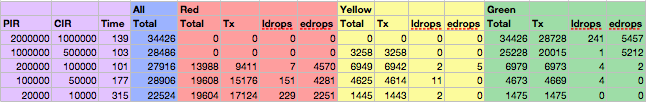
\includegraphics[width=120mm]{images/punkt_3_tabela.png}

\paragraph{}
Zadaniem administratora sieci jest takie wypośrodkowanie ustawień aby w razie przeciążenia wszystkie kolejki pracowały, zachowując odpowiednie proporcje ilości pakietów.
Wnioski

\paragraph{}
DiffServ jest jednym z wielu rozwiązań pozwalającym administratorom na dostosowanie sieci do wymogów biznesowych. Pozwala zapewnić odpowiednie parametry jakości obsługi dzięki szczegółowej konfiguracji zachowania węzłów jak i połączeń. Jego obszar aplikacji to większe sieci składające się z dużej ilości urządzeń w których skład wchodzą routery brzegowe i szkieletowe.

\paragraph{}
Aby skonfigurować działąjący system QoS musieliśmy zadać sobie dużo trudu, nie polecamy więć systemu DiffServe dla początkujących administratorów.




\end{document}


